% !TeX program = lualatex
\documentclass[aspectratio=1610]{beamer}

\title{AI Project: Connect Four}
\subtitle{Minimax Algorithm Analysis}
\date{SS~2026}
\author{Martin Scheuchenpflug \and Niklas Etzlinger}
\institute{Artificial Intelligence --- FH Upper Austria}

\usetheme[numbering=progressbar, pattern=triangleiso, sectionpage=none]{wildcat}

\usepackage{booktabs}
\usepackage{listings}
\lstset{
  language=Java,
  basicstyle=\ttfamily\scriptsize,
  keywordstyle=\bfseries,
  backgroundcolor=\color{wcprimary10},
  frame=single, framerule=0pt,
  breaklines=true,
  xleftmargin=0.5em, xrightmargin=0.5em,
}

\graphicspath{{./images/}}

%%%------------------------------------------------------------
\begin{document}
%%%------------------------------------------------------------

\begin{frame}
  \titlepage
\end{frame}



%%%------------------------------------------------------------
\section{Setup \& Original Version (Q1)}
%%%------------------------------------------------------------

\begin{frame}{Experimental Setup}
  \begin{columns}[T]
    \column{0.48\textwidth}
      \begin{block}{Game}
        \begin{itemize}
          \item Connect Four on a $6 \times 8$ board (later: $6 \times 7$)
          \item Computer plays as \textbf{second player} (red)
          \item Fixed \textbf{search depth:~4}
        \end{itemize}
      \end{block}
      \begin{block}{Metric}
        Number of board positions the computer examines before choosing its move
        (logged as \emph{``moves tried''}).
      \end{block}
    \column{0.48\textwidth}
      \begin{alertblock}{Six variants measured}
        \begin{itemize}
          \item Q1 — original (shallow $\alpha$-$\beta$)
          \item Q2 — pure minimax (no pruning)
          \item Q3 — equal-value cutoffs ($\geq$/$\leq$)
          \item Q4 — deep $\alpha$-$\beta$
          \item Q5a — pure minimax + middle-out
          \item Q5b — deep $\alpha$-$\beta$ + middle-out
        \end{itemize}
      \end{alertblock}
  \end{columns}
\end{frame}

\begin{frame}{The Game: Connect Four}
  \begin{figure}
    \centering
    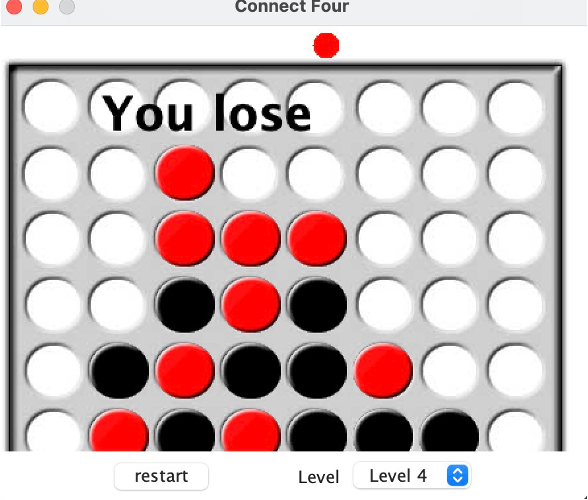
\includegraphics[height=0.75\textheight]{Game}
  \end{figure}
\end{frame}

\begin{frame}{Q1: Shallow $\alpha$-$\beta$ Pruning}
  \begin{columns}[T]
    \column{0.55\textwidth}
      \begin{block}{How it works}
        Each recursive call passes only the \emph{direct parent's} current best value as a bound.
        Bounds from grandparents and higher are silently discarded.
      \end{block}
      \vspace{0.4em}
      \begin{itemize}
        \item \textbf{Max node} prunes if child strength $>$ parent min's current minimum
        \item \textbf{Min node} prunes if child strength $<$ parent max's current maximum
        \item Ancestors offer \emph{no} additional tightening
      \end{itemize}
    \column{0.42\textwidth}
      \begin{exampleblock}{Measured move counts}
        \centering\small
        \begin{tabular}{cc}
          \toprule
          Move & Q1 \\
          \midrule
          1 & 1426 \\
          2 &  925 \\
          3 &  654 \\
          4 &  809 \\
          5 & 1221 \\
          \bottomrule
        \end{tabular}
      \end{exampleblock}
      Range: $\approx 650$ – $2{,}459$ depending on board state.
  \end{columns}
\end{frame}

%%%------------------------------------------------------------
\section{Pure Minimax --- No Pruning (Q2)}
%%%------------------------------------------------------------

\begin{frame}[fragile]{Q2: Removing All Pruning}
  \begin{columns}[T]
    \column{0.52\textwidth}
      \begin{block}{Code change}
        Both cutoff blocks were commented out:
      \end{block}
      \begin{lstlisting}
// in expandMaxNode:
// if (strength > parentMinimum) {
//   board.undoLastMove();
//   return strength;
// }

// in expandMinNode:
// if (strength < parentMaximum) {
//   board.undoLastMove();
//   return strength;
// }
      \end{lstlisting}
    \column{0.44\textwidth}
      \begin{alertblock}{Effect}
        Every node in the search tree is expanded — no cutoffs at all.
      \end{alertblock}
      \vspace{0.4em}
      \begin{block}{Theoretical count (depth $d$, branching $n$)}
        \[
          \text{total}(d) = \frac{n^{d+1} - n}{n - 1}
        \]
        For $n = 8,\ d = 4$:
        \[
          \frac{8^5 - 8}{7} = \frac{32760}{7} = \mathbf{4680}
        \]
      \end{block}
      First three moves all measured \textbf{exactly 4680}.
  \end{columns}
\end{frame}

%%%------------------------------------------------------------
\section{Equal-Value Pruning (Q3)}
%%%------------------------------------------------------------

\begin{frame}[fragile]{Q3: Pruning on Equal Values}
  \begin{columns}[T]
    \column{0.50\textwidth}
      \begin{block}{Original (strict)}
        A value \emph{equal} to the bound does not trigger a cutoff.
      \end{block}
      \begin{lstlisting}
// max node
if (strength > parentMinimum) return;
// min node
if (strength < parentMaximum) return;
      \end{lstlisting}
      \vspace{0.3em}
      \begin{block}{Q3: equal cutoff}
        An equality does trigger a cutoff too.
      \end{block}
      \begin{lstlisting}
// max node — fires on tie too
if (strength >= parentMinimum) return;
// min node — fires on tie too
if (strength <= parentMaximum) return;
      \end{lstlisting}
    \column{0.46\textwidth}
      \begin{exampleblock}{Why it helps}
        The heuristic assigns identical scores to many symmetric positions early in the game.
        Pruning on equality eliminates entire subtrees that the strict version still explores.
      \end{exampleblock}
      \vspace{0.4em}
      \begin{alertblock}{Result}
        Move counts drop consistently vs Q1.\\[0.3em]
        Example: move~1 drops from \textbf{1426} (Q1) to \textbf{1208} (Q3).
      \end{alertblock}
  \end{columns}
\end{frame}

%%%------------------------------------------------------------
\section{Deep $\alpha$-$\beta$ (Q4)}
%%%------------------------------------------------------------

\begin{frame}{Q4: Deep $\alpha$-$\beta$ --- Motivation}
  \begin{columns}[T]
    \column{0.48\textwidth}
      \begin{block}{Shallow (Q1/Q3)}
        \centering\vspace{0.4em}
        \begin{tikzpicture}[
          every node/.style={draw, rounded corners, minimum width=1.1cm,
                             minimum height=0.42cm, font=\scriptsize},
          >=stealth, scale=0.9]
          \node[fill=wcprimary20] (root) at (0, 0)    {MAX};
          \node[fill=wcprimary10] (min1) at (-1.4,-1.1) {MIN};
          \node[fill=wcprimary10] (min2) at ( 1.4,-1.1) {MIN};
          \node[fill=gray!20]     (max1) at (-1.4,-2.2) {MAX};
          \node[fill=gray!20]     (max2) at ( 1.4,-2.2) {MAX};
          \draw[->] (root) -- node[draw=none,left,font=\tiny] {local $\alpha$} (min1);
          \draw[->] (root) -- (min2);
          \draw[->] (min1) -- node[draw=none,left,font=\tiny] {local $\beta$} (max1);
          \draw[->] (min2) -- (max2);
        \end{tikzpicture}\\[0.4em]
        \footnotesize Each node passes only its \emph{own} value — ancestor bounds are lost.
      \end{block}
    \column{0.48\textwidth}
      \begin{alertblock}{Deep (Q4)}
        \centering\vspace{0.4em}
        \begin{tikzpicture}[
          every node/.style={draw, rounded corners, minimum width=1.1cm,
                             minimum height=0.42cm, font=\scriptsize},
          >=stealth, scale=0.9]
          \node[fill=wcprimary20] (root) at (0, 0)    {MAX};
          \node[fill=wcprimary10] (min1) at (-1.4,-1.1) {MIN};
          \node[fill=wcprimary10] (min2) at ( 1.4,-1.1) {MIN};
          \node[fill=gray!20]     (max1) at (-1.4,-2.2) {MAX};
          \node[fill=gray!20]     (max2) at ( 1.4,-2.2) {MAX};
          \draw[->] (root) -- node[draw=none,left,font=\tiny]  {$\alpha,\beta$} (min1);
          \draw[->] (root) -- node[draw=none,right,font=\tiny] {$\alpha,\beta$} (min2);
          \draw[->] (min1) -- node[draw=none,left,font=\tiny]  {$\alpha,\beta$} (max1);
          \draw[->] (min2) -- node[draw=none,right,font=\tiny] {$\alpha,\beta$} (max2);
        \end{tikzpicture}\\[0.4em]
        \footnotesize Both $\alpha$ and $\beta$ thread through the \emph{whole} tree — every node sees the tightest window from \textbf{all} ancestors.
      \end{alertblock}
  \end{columns}
\end{frame}

\begin{frame}[fragile]{Q4: Deep $\alpha$-$\beta$ --- Code}
  \begin{lstlisting}
private int expandMaxNode(int depth, int alpha, int beta) {
    for each move:
        int strength = expandMinNode(depth - 1, alpha, beta); // pass both down
        if (strength >= beta)  { board.undoLastMove(); return strength; } // beta cutoff
        if (strength > maxStrength) maxStrength = strength;
        if (strength > alpha) alpha = strength; // tighten alpha for next sibling
}
private int expandMinNode(int depth, int alpha, int beta) {
    for each move:
        int strength = expandMaxNode(depth - 1, alpha, beta); // pass both down
        if (strength <= alpha) { board.undoLastMove(); return strength; } // alpha cutoff
        if (strength < minStrength) minStrength = strength;
        if (strength < beta) beta = strength;  // tighten beta for next sibling
}
  \end{lstlisting}
  \begin{exampleblock}{Effect}
    Move~1: \textbf{993} (vs 1208 in Q3).
    Tightening at any level immediately benefits \emph{all} descendants.
  \end{exampleblock}
\end{frame}

%%%------------------------------------------------------------
\section{Move-Ordering Heuristic (Q5)}
%%%------------------------------------------------------------

\begin{frame}[fragile]{Q5: Middle-Out Move Ordering}
  \begin{columns}[T]
    \column{0.50\textwidth}
      \begin{block}{Idea}
        $\alpha$-$\beta$ is most effective when the \emph{best} moves come first.\\[0.3em]
        In Connect Four, centre columns are generally stronger.\\
        $\Rightarrow$ Try them first.
      \end{block}
      \begin{lstlisting}
private static final int[] COLUMN_ORDER 
= {3, 2, 4, 1, 5, 0, 6};
private Move[] reorder(Move[] moves) {
    Move[] ordered = new Move[moves.length];
    for (int i = 0; i < COLUMN_ORDER.length; i++)
        ordered[i] = moves[COLUMN_ORDER[i]];
    return ordered;
}
      \end{lstlisting}
      Called at all three loop sites: \texttt{calculateMove}, \texttt{expandMaxNode}, \texttt{expandMinNode}.
    \column{0.46\textwidth}
      \begin{block}{Q5a — pure minimax + middle-out}
        Without pruning, traversal order does \textbf{not} affect node count.\\
        Counts stay close to 4680 (same formula as Q2).\\[0.3em]
        \footnotesize Minor deviations: different move choices lead to slightly different board states.
      \end{block}
      \vspace{0.3em}
      \begin{alertblock}{Q5b — deep $\alpha$-$\beta$ + middle-out}
        Move~1: \textbf{302} (vs 993 in Q4).\\[0.3em]
        Best columns first $\Rightarrow$ tight window established immediately $\Rightarrow$ remaining columns pruned early.
      \end{alertblock}
  \end{columns}
\end{frame}

%%%------------------------------------------------------------
\section{Results}
%%%------------------------------------------------------------

\begin{frame}{Results: All Variants at Depth 4}
  \centering
  \footnotesize
  \begin{tabular}{r rrrrrr}
    \toprule
    \textbf{Move} &
    \textbf{Q1} &
    \textbf{Q2} &
    \textbf{Q3} &
    \textbf{Q4} &
    \textbf{Q5a} &
    \textbf{Q5b} \\
    & \scriptsize original &
    \scriptsize pure minimax &
    \scriptsize ${\geq}$ prune &
    \scriptsize deep $\alpha$-$\beta$ &
    \scriptsize pure+order &
    \scriptsize deep+order \\
    \midrule
     1 & 1426 & 4680 & 1208 &  993 & 4680 &  302 \\
     2 &  925 & 4680 &  771 &  642 & 4680 &  360 \\
     3 &  654 & 4680 &  574 &  514 & 4650 &  702 \\
     4 &  809 & 4623 &  745 &  612 & 4538 &  899 \\
     5 & 1221 & 4622 & 1158 &  934 & 4650 &  872 \\
     6 & 2459 & 4056 & 2007 & 1936 & 4649 &  773 \\
     7 &  909 & 4544 &  854 &  754 & 4333 &  785 \\
     8 &  760 & 4256 &  736 &  664 & 4325 &  671 \\
     9 &  899 & 3978 &  793 &  665 & 2792 &  305 \\
    10 &  664 & 3641 &   59 &   59 & 2347 &   95 \\
    \midrule
    \textbf{SUM} & \textbf{10726} & \textbf{43760} & \textbf{8905} & \textbf{7773} & \textbf{41644} & \textbf{5764} \\
    \bottomrule
  \end{tabular}

  \vspace{0.4em}
  \normalsize
  Q5b (\textbf{5764}) examines \textbf{7.6$\times$ fewer} positions than Q2 (43760) and
  \textbf{1.9$\times$ fewer} than Q1 (10726).
  For Q1-Q4 the palyer moves were equal, at Q5a and Q5b the player's moves had to be adopted to not loose in < 10 moves.
\end{frame}

\begin{frame}{Results: Visual Comparison}
  \begin{figure}
    \centering
    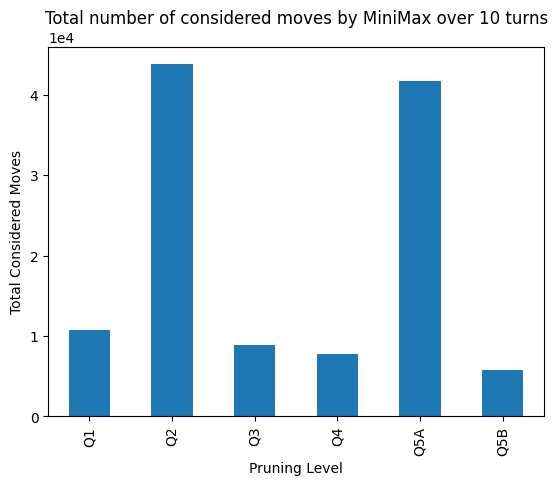
\includegraphics[height=0.75\textheight]{PruningResult}
  \end{figure}
  \footnotesize
  Q2 and Q5a (no pruning) dominate. Each pruning step reduces counts; Q5b achieves the lowest.
\end{frame}

%%%------------------------------------------------------------
\section{7-Column Board (Q6)}
%%%------------------------------------------------------------

\begin{frame}[fragile]{Q6: Reducing to 7 Columns}
  \begin{columns}[T]
    \column{0.48\textwidth}
      \begin{block}{Change the constant}
        \begin{lstlisting}
// C4Board.java
public static final int NUMBER_OF_COLUMNS = 7;
        \end{lstlisting}
        All array sizes and loop bounds are derived from this constant.
      \end{block}
      \begin{block}{Update move-ordering array}
        \begin{lstlisting}
// 7-column centre-out
private static final int[] COLUMN_ORDER =
    {3, 2, 4, 1, 5, 0, 6};
        \end{lstlisting}
      \end{block}
    \column{0.48\textwidth}
      \begin{alertblock}{Magic number 84}
        One literal not derived from constants:
        \begin{lstlisting}
rows = new Vector<C4Row>(84);
        \end{lstlisting}
        84 = four-slot groups on a $6\times8$ board.
      \end{alertblock}
      \begin{exampleblock}{Formula: $R(C{-}3)+(R{-}3)C+2(R{-}3)(C{-}3)$}
        \scriptsize\centering
        \begin{tabular}{lcc}
          \toprule
          Direction & $6{\times}8$ & $6{\times}7$ \\
          \midrule
          Horizontal  & 30 & 24 \\
          Vertical    & 24 & 21 \\
          Diagonals   & 30 & 24 \\
          \midrule
          \textbf{Total} & \textbf{84} & \textbf{69} \\
          \bottomrule
        \end{tabular}
      \end{exampleblock}
  \end{columns}
\end{frame}

%%%------------------------------------------------------------
\section{Heuristic Evaluation Function (Q7)}
%%%------------------------------------------------------------

\begin{frame}[fragile]{Q7: What the Heuristic Counts}
  \begin{columns}[T]
    \column{0.50\textwidth}
      \begin{block}{Open groups}
        A group of 4 consecutive slots containing tokens of \emph{only one} player.\\
        (Mixed groups are dead — counted for neither player.)
      \end{block}
      \vspace{0.3em}
      Tracked separately: open groups of size \textbf{1}, \textbf{2}, \textbf{3}.
      \vspace{0.3em}
      \begin{lstlisting}
// SHIFT_3_IN_A_ROW = 5  =>  x32
// SHIFT_2_IN_A_ROW = 2  =>  x4
return (p1_3InARow << 5)
     + (p1_2InARow << 2)
     + p1_1InARow;
      \end{lstlisting}
      Weights: \textbf{32 : 4 : 1}
    \column{0.46\textwidth}
      \begin{alertblock}{Special cases}
        \begin{itemize}
          \item 4-in-a-row $\Rightarrow$ \texttt{Integer.MAX\_VALUE} (win)
          \item Opponent has 4-in-a-row $\Rightarrow$ raw strength = 0
        \end{itemize}
      \end{alertblock}
      \vspace{0.3em}
      \begin{exampleblock}{Final heuristic value}
        \[
          \texttt{getStrength}(p)
            = \text{str}_{p} - \text{str}_{\text{opp}}
        \]
        Positive = good for player $p$,\\
        negative = bad.
      \end{exampleblock}
  \end{columns}
\end{frame}

\begin{frame}{Q7: Observer Pattern --- Incremental O(1) Evaluation}
  \begin{columns}[T]
    \column{0.48\textwidth}
      \begin{block}{C4Slot (Subject)}
        \footnotesize
        \begin{itemize}
          \item Holds one cell's content
          \item Fires \texttt{contentsChanged()} to all listeners on every write
        \end{itemize}
      \end{block}
      \begin{block}{C4Row (Observer)}
        \footnotesize
        \begin{itemize}
          \item Represents one group of 4 consecutive slots
          \item Registered on all 4 slots at construction
          \item Updates group counters, calls \texttt{Inc}/\texttt{Dec} on the shared \texttt{C4Stats} accumulator — board-wide counters updated in \textbf{O(1)}
        \end{itemize}
      \end{block}
    \column{0.48\textwidth}
      \begin{exampleblock}{Call chain on every move}
        \footnotesize
        \texttt{board.move()}\\
        \quad $\to$ \texttt{slot.setContents(n)}\\
        \quad\quad $\to$ notifies each \texttt{C4Row}\\
        \quad\quad\quad $\to$ \texttt{row.contentsChanged()}\\
        \quad\quad\quad\quad $\to$ \texttt{stats.pX\_NInARowInc()}
      \end{exampleblock}
      \vspace{0.4em}
      \texttt{undoLastMove()} triggers the same chain in \emph{reverse} — no board scan needed.
      \vspace{0.4em}
      \begin{block}{Why it matters}
        \footnotesize
        Each \texttt{board.move()} and \texttt{undoLastMove()} costs O(1) for the heuristic — no full board scan at every minimax node.
      \end{block}
  \end{columns}
\end{frame}

%%%------------------------------------------------------------
\section{Missing the Immediate Win (Q8)}
%%%------------------------------------------------------------

\begin{frame}[fragile]{Q8: Why the Computer Misses the Immediate Win}
  \begin{columns}[T]
    \column{0.52\textwidth}
      \begin{alertblock}{Root cause}
        \footnotesize Every win scores \texttt{Integer.MAX\_VALUE} regardless of depth — a win in 1 move and a win in 3 moves look \emph{identical}.
      \end{alertblock}
      \begin{block}{Move-selection loop}
        \begin{lstlisting}
if (strength > maxStrength) {
    maxStrength = strength;
    maxIndex = i;
}
        \end{lstlisting}
        \footnotesize Updates only on a \emph{strict} improvement — ties are ignored.
      \end{block}
    \column{0.44\textwidth}
      \begin{block}{Scenario (left-to-right ordering)}
        \begin{enumerate}\footnotesize
          \item Col~0 tried first — search finds a forced win 3 moves deep. Returns \texttt{MAX\_VALUE}. \texttt{maxIndex = 0}.
          \item Col~3 is the immediate win. Also returns \texttt{MAX\_VALUE}.
          \item \texttt{MAX\_VALUE > MAX\_VALUE} is \textbf{false} — \texttt{maxIndex} stays at 0.
          \item Computer plays col~0: wins, but not immediately.
        \end{enumerate}
      \end{block}
      \begin{exampleblock}{Potential Fix}
        \footnotesize Encode depth in the score: \texttt{MAX\_VALUE\,$-$\,depth}, so shallower wins always outrank deeper ones.
      \end{exampleblock}
  \end{columns}
\end{frame}

%%%------------------------------------------------------------

\standout{Summary}

\begin{frame}{Summary}
  \begin{columns}[T]
    \column{0.48\textwidth}
      \begin{block}{Pruning progression}
        \begin{tabular}{lrl}
          Q2 (no pruning)  & 43\,760 &  $100\%$ \\
          Q1 (shallow $\alpha$-$\beta$) & 10\,726 & $-75\%$ \\
          Q3 (equal cuts)             &  8\,905 & $-79\%$ \\
          Q4 (deep $\alpha$-$\beta$)  &  7\,773 & $-82\%$ \\
          Q5b (+ ordering) &  5\,764 & $-87\%$ \\
        \end{tabular}
      \end{block}
      \vspace{0.3em}
      Move ordering (Q5b) gives the \textbf{largest single reduction}:
      good columns first $\Rightarrow$ tight window $\Rightarrow$ massive pruning.
    \column{0.48\textwidth}
      \begin{exampleblock}{Key takeaways}
        \begin{itemize}
          \item Pure minimax visits $\frac{n^{d+1}-n}{n-1}$ nodes — exponential in depth
          \item Every pruning refinement compounds the savings
          \item Move ordering \emph{without} pruning is irrelevant (Q5a $\approx$ Q2)
          \item A single constant controls board size; one magic number needed a formula
          \item Flat win scores cause occasional missed immediate wins
        \end{itemize}
      \end{exampleblock}
  \end{columns}
\end{frame}

%%%------------------------------------------------------------
\end{document}
%%%------------------------------------------------------------
